\documentclass[tikz]{standalone}
\usepackage{fancyvrb}
\usetikzlibrary{decorations.pathreplacing,calligraphy,positioning,calc,arrows.meta}
\begin{document}
\newcommand{\dbitem}[2]{
    \begin{minipage}{0.7cm}
        \centering{#1}
        \linebreak
        \centering{\##2}
    \end{minipage}
}

\newcommand{\dbitemlbl}[1]{
    \rotatebox{-90}{\color{darkgray}\footnotesize #1}
}
\newcommand\dddots{\makebox[1em][c]{.\hfil.\hfil.}}
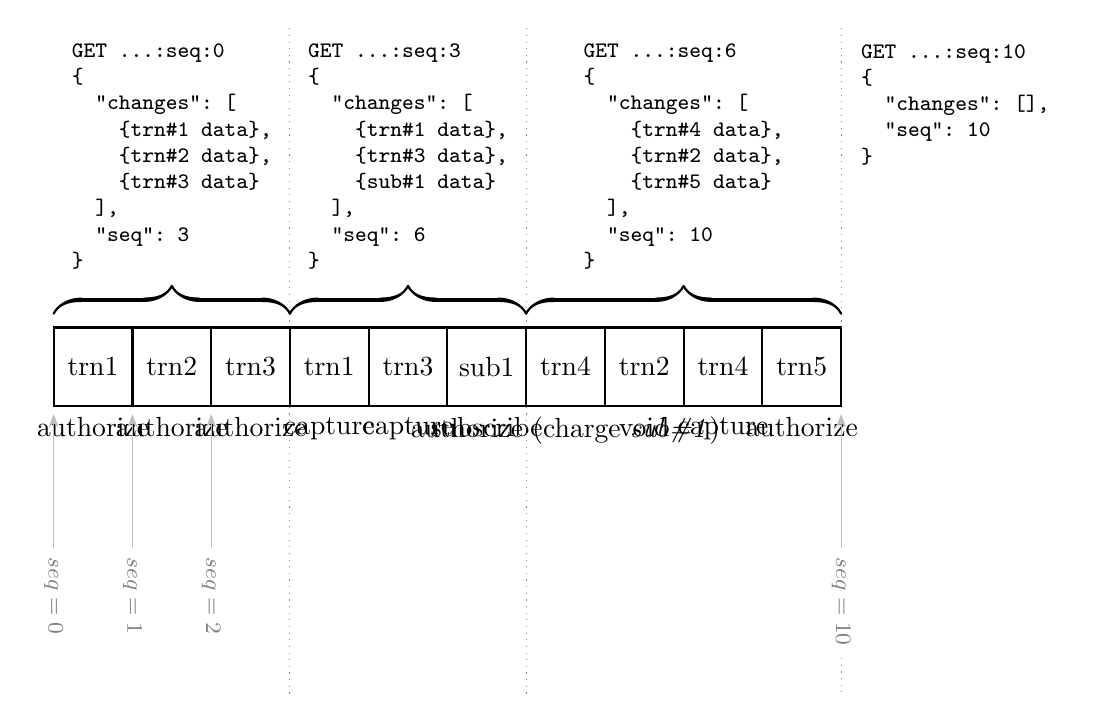
\begin{tikzpicture}
\tikzstyle{DBitem} = [draw=black, thick, minimum width=1cm, minimum height=1cm, node distance=1cm]
\tikzstyle{Seqcall} = [draw=none, minimum width=3cm, anchor=north, node distance=0.6cm]
\node [name=s1,              DBitem, label=below:{\dbitemlbl{authorize}}] {\dbitem{trn}{1}};
\node [name=s2, right of=s1, DBitem, label=below:{\dbitemlbl{authorize}}] {\dbitem{trn}{2}};
\node [name=s3, right of=s2, DBitem, label=below:{\dbitemlbl{authorize}}] {\dbitem{trn}{3}};
\draw [dotted, draw=gray] (2.5,4.3) -- (2.5,-4.2);
\node [name=s4, right of=s3, DBitem, label=below:{\dbitemlbl{capture}}] {\dbitem{trn}{1}};
\node [name=s5, right of=s4, DBitem, label=below:{\dbitemlbl{capture}}] {\dbitem{trn}{3}};
\node [name=s6, right of=s5, DBitem, label=below:{\dbitemlbl{subscribe}}] {\dbitem{sub}{1}};
\draw [dotted, draw=gray] (5.5,4.3) -- (5.5,-4.2);
\node [name=s7, right of=s6, DBitem, label=below:{\dbitemlbl{authorize (charge \textit{sub\#1})}}] {\dbitem{trn}{4}};
\node [name=s8, right of=s7, DBitem, label=below:{\dbitemlbl{void}}] {\dbitem{trn}{2}};
\node [name=s9, right of=s8, DBitem, label=below:{\dbitemlbl{capture}}] {\dbitem{trn}{4}};
\node [name=s10, right of=s9, DBitem, label=below:{\dbitemlbl{authorize}}] {\dbitem{trn}{5}};
\draw [dotted, draw=gray] (9.5,4.3) -- (9.5,0.5);
\draw [dotted, draw=gray] (9.5,-3.7) -- (9.5,-4.2);
\draw [decorate, ultra thick, decoration = {calligraphic brace,raise=5pt,amplitude=10pt}] (-0.5,0.5) -- (2.5,0.5);
\draw [decorate, ultra thick, decoration = {calligraphic brace,raise=5pt,amplitude=10pt}] (2.5,0.5) -- (5.5,0.5);
\draw [decorate, ultra thick, decoration = {calligraphic brace,raise=5pt,amplitude=10pt}] (5.5,0.5) -- (9.5,0.5);
\node [Seqcall, above=of s2] {
\footnotesize\begin{BVerbatim}
GET ...:seq:0
{
  "changes": [
    {trn#1 data},
    {trn#2 data},
    {trn#3 data}
  ],
  "seq": 3
}
\end{BVerbatim}
};
\node [Seqcall, above=of s5] {
\footnotesize\begin{BVerbatim}
GET ...:seq:3
{
  "changes": [
    {trn#1 data},
    {trn#3 data},
    {sub#1 data}
  ],
  "seq": 6
}
\end{BVerbatim}
};
\node [Seqcall, name=lastseq, above=of $(s8.north)!0.5!(s9.north)$] {
\footnotesize\begin{BVerbatim}
GET ...:seq:6
{
  "changes": [
    {trn#4 data},
    {trn#2 data},
    {trn#5 data}
  ],
  "seq": 10
}
\end{BVerbatim}
};
\node [Seqcall, right of=lastseq, node distance=3.45cm] {
\footnotesize\begin{BVerbatim}
GET ...:seq:10
{
  "changes": [],
  "seq": 10
}




\end{BVerbatim}
};
\draw [-Stealth, text=gray, draw=lightgray] (-0.5,-2.3) node[below,anchor=west,rotate=-90] {\footnotesize $seq=0$} -- (-0.5,-0.6);
\draw [-Stealth, text=gray, draw=lightgray] (0.5,-2.3) node[below,anchor=west,rotate=-90] {\footnotesize $seq=1$} -- (0.5,-0.6);
\draw [-Stealth, text=gray, draw=lightgray] (1.5,-2.3) node[below,anchor=west,rotate=-90] {\footnotesize $seq=2$} -- (1.5,-0.6);
\draw [-Stealth, text=gray, draw=lightgray] (9.5,-2.3) node[below,anchor=west,rotate=-90] {\footnotesize $seq=10$} -- (9.5,-0.6);
\end{tikzpicture}
\end{document}
